\chapter{Present literature}
\label{chpr:ch2}
\bigskip
In literature we still can find few studies about the correlations inside the world of cryptoassets.

Cryptoassets market has grown continuously through the years: since the born of Bitcoin a lot of new coins have been launched and all of them have been increasingly exchanged during time.
Figure \ref{mc_allcrypto} shows the market capitalization of all the cryptoasset taken from \href{https://coinmarketcap.com/it/charts/}{coinmarketcap.com}. 

\begin{figure}[htpb]
		\centering
		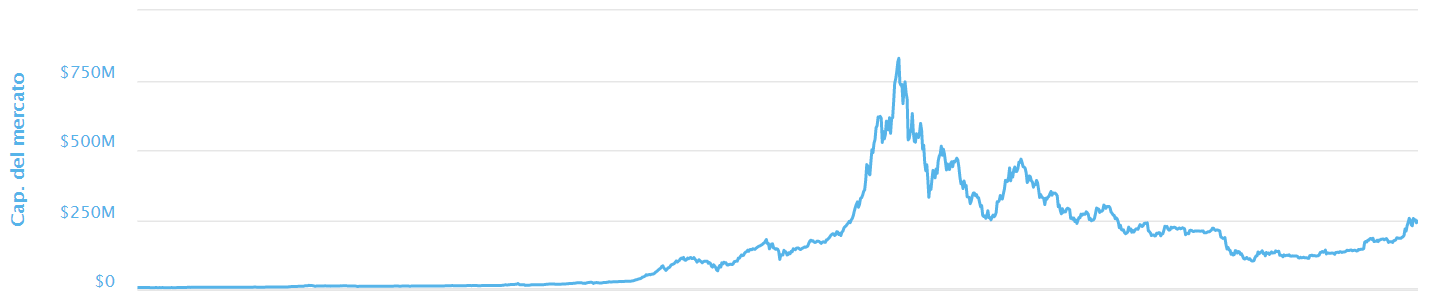
\includegraphics[width=13cm]{Images/mktcap.png} %
		\caption{Market Cap of the cryptocurrencys (source: \href{https://coinmarketcap.com/it/charts/}{coinmarketcap.com})}
		\label{mc_allcrypto}
\end{figure}
\bigskip
\noindent
The value reached between the last years suggests that they may be seen as a new category of investment assets.

For this reason one may wonder if there are properties which characterize this new asset-class.
As the bond market is considered a hedging against bad times for stock markets, or the gold is considered a safe haven where to keep money safe from volatility it’s interesting to investigate if this kind of properties hold also for cryptoassets.

\newpage
\section{Asset Class}
In \citep{corbet} there is one of the first attempt to analyse these properties. Authors considered the returns of Bitcoin, Litecoin and Ripple to represent cryptoassets and other indexes to represent all the other asset classes: MSC GSCI Total Returns Index, the US\$ Broad Exchange Rate, the SP500 Index and the COMEX closing gold price, VIX and the Markit ITTR110 index. All the data where collected in a period from January 2013 to July 2017, that is just before the well-known rally of bitcoin that pushed its price near to 20’000\$.
Authors focused on studying spillover indexes both in time and frequency domain between all the instruments in the dataset. They found that cryptoassets are highly connected to each other and disconnected from mainstream assets. Their results also support the position that cryptocurrency market is a new investment asset class, since they are interconnected with each other and have similar patterns of connectedness with other asset classes.

It’s still necessary to go deeper in the analysis: cryptoassets can be considered a new asset-class but it’s necessary to keep in mind that this is a “young” market and correlations may vary over time.

For example, in \citep{weiyi} a further study on the diversification between cryptoassets is performed. The dataset considered includes Bitcoin, Ethereum, Ripple, Litecoin, Stellar, Monero, Dash, Tether, NEM and Verge, and it covers the period from 07-Aug-15 to 09-Apr-18, that contains the rally previously stated and also the come-back (to 7’000\$ for bitcoin).

By using this time window the authors observe that the highest correlation is between Bitcoin and Litecoin and it’s just 0.52. Globally they get very low correlations between cryptocurrencies as shown in figure \ref{corr_i}:
\begin{figure}[H]
		\centering
		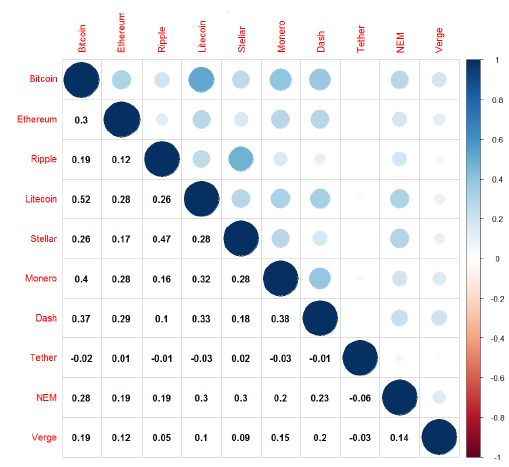
\includegraphics[width=10cm]{Images/corrs_wei.png} %
		\caption{Correlation Matrix for cryptocurrencies, source: \citep{weiyi}}
		\label{corr_i}
\end{figure}
\bigskip

\noindent
Then, authors proceed by performing the efficient frontier of a portfolio composed with all of these cryptoassets and then by looking for the optimal allocation. To get it, they use different methods that are summarized in table \ref{tab_21}:

\begin{table}[H]
    \begin{tabular}{p{2.5cm}|p{4.4cm}|p{1.9cm}|p{3cm}}
    Model & Objective Function & Type & Constraints \\
    \hline
    \(\displaystyle 1/N -  Rule\) & - & - & - \\ \hline
    Minimum Variance & \(\displaystyle w'\Sigma w\) & Minimize & \(\displaystyle w'\mathbb{1} w=1, w \geq 0 \) \\ \hline
    Risk Parity & \(\displaystyle \sum_{{i=1}}^{N} \left[w_i \left(\Sigma w\right)_i-w'\Sigma w/N\right] \) & Minimize & \(\displaystyle w'\mathbb{1} w=1, w\geq 0 \) \\ \hline
    Markowitz & \(\displaystyle w'\Sigma w \) & Minimize & \(\displaystyle w'\mu\geq\mu_0, w'\mathbb{1} w=1, w\geq 0 \) \\ \hline
    Maximum Sharpe & \(\displaystyle w'\mu /\sqrt{w'\Sigma w} \) & Maximize & \(\displaystyle w'\mathbb{1} w=1, w\geq 0 \) \\   \hline
    Maximum Utility & \(\displaystyle w'\mu - \frac{\gamma}{2}w'\Sigma w \) & Maximize & \(\displaystyle w'\mathbb{1} w=1, w\geq 0 \) \\
    \hline
    \end{tabular}
    \caption{Models used  in the paper}
    \label{tab_21}
\end{table}

\bigskip
$\mu_0$ in the Markowitz model is set to be the corresponding mean under 1/N-Rule, and the risk aversion parameter γ is 1 in the maximum utility model.
The authors show that almost any of that models can beat the 1/N-Rule in terms of Sharp ratio.
This result is, of course, due to the low correlations between cryptoassets but, as we said, they depend on the time period one considers. Further considerations on these results are discussed in chapter \ref{chpr:ch3}.

\section{Optimal Allocation}
More research has been done about the usage of bitcoin in an investment portfolio to diversify and reach higher returns. A contribution has been given in \citep{samuele}.

In that work the author starts by studying the correlation of Bitcoin with some index representative of the market. Then, given that Bitcoin turns out to be uncorrelated with the market, he performs optimal portfolio allocation analyses to investigate its diversification properties, both with Markowitz mean-variance optimization and with the CVaR as portfolio risk measure. Evidence shows that allocating a small percentage of wealth in the digital assets proves to be extremely beneficial in terms of lowering the risk and increasing the expected returns.

The dataset considered is composed by the same instruments we consider in our thesis in order to explore the relation of Bitcoin with all the possible asset classes. Differently from us, the period he considers is from the $19^{th}$ of July 2010 till the $2^{nd}$ of November 2018.

First, the author assess the correlation of the cryptoasset with the indexes by observing the historical correlation of the daily returns.

\begin{table}[H]
    \resizebox{\textwidth}{!}{\begin{tabular}{c c c c c c c c c c c c c c c c c}
       &
       \rotatebox[origin=c]{45}{btc} & \rotatebox[origin=c]{45}{bric} & \rotatebox[origin=c]{45}{sp500} & \rotatebox[origin=c]{45}{eurostoxx} & \rotatebox[origin=c]{45}{nasdaq} & \rotatebox[origin=c]{45}{bond\_europe} & \rotatebox[origin=c]{45}{bond\_us} & \rotatebox[origin=c]{45}{bond\_eur} & \rotatebox[origin=c]{45}{eur} & \rotatebox[origin=c]{45}{gbp} & \rotatebox[origin=c]{45}{chf} & \rotatebox[origin=c]{45}{jpy} & \rotatebox[origin=c]{45}{gold} & \rotatebox[origin=c]{45}{wti} & \rotatebox[origin=c]{45}{grain} & \rotatebox[origin=c]{45}{metal} \\ \hline
        btc & 1.0 & 1.4 & 4.4 & 4.1 & 3.6 & 1.4 & -1.8 & 1.9 & 2.3 & 0.7 & 2.5 & -1.1 & -0.2 & 0.8 & 3.5 & 2.7\\
    \end{tabular}}
    \caption{Historical Correlations between bitcoin and other instruments, source: \citep{samuele}}
\end{table}
\bigskip
After that he calibrate several more sophisticated models and look for the correlations in these models.
The first is the Jump Diffusion model presented in 1976 by R.C. Merton where log-normal jumps are added to the simple Black\&Scholes dynamics of the asset price.

\begin{equation}
  \frac{dS_t}{S_t} = \left(\mu - \lambda\mu_J \right) dt + \sigma dW_t + Y_t dN ,  
\end{equation}

The results are showed in the following table:

\begin{table}[H]
    \resizebox{\textwidth}{!}{\begin{tabular}{c c c c c c c c c c c c c c c c c}
       &
       \rotatebox[origin=c]{45}{btc} & \rotatebox[origin=c]{45}{bric} & \rotatebox[origin=c]{45}{sp500} & \rotatebox[origin=c]{45}{eurostoxx} & \rotatebox[origin=c]{45}{nasdaq} & \rotatebox[origin=c]{45}{bond\_europe} & \rotatebox[origin=c]{45}{bond\_us} & \rotatebox[origin=c]{45}{bond\_eur} & \rotatebox[origin=c]{45}{eur} & \rotatebox[origin=c]{45}{gbp} & \rotatebox[origin=c]{45}{chf} & \rotatebox[origin=c]{45}{jpy} & \rotatebox[origin=c]{45}{gold} & \rotatebox[origin=c]{45}{wti} & \rotatebox[origin=c]{45}{grain} & \rotatebox[origin=c]{45}{metal} \\ \hline
        btc & 1.0 & 2.7 & 7.7 & 6.3 & 6.4 & 1.9 & -2.4 & 2.7 & 2.7 & 1.2 & 4.4 & -1.8 & -0.6 & 1.1 & 4.2 & 4.2\\
    \end{tabular}}
    \caption{Correlations under Jump Diffusion model, source: \citep{samuele}}
\end{table}
\bigskip

Then the stochastic volatility (SV) model of Heston (1993) is presented and calibrated. This model introduced a new stochastic process that accounts for the variance of the underlying price which evolves as in B\&S but with a stochastic volatility term.

\begin{equation}
  \frac{dS_t}{S_t} = \mu dt + \sqrt{V_T}dW_t^S  ,
\end{equation}
\begin{equation}
  dV_t = k\left(\Theta - V_t \right) dt + \sigma _V \sqrt{Vt}dW_t^V ,
\end{equation}
\begin{table}[H]
    \resizebox{\textwidth}{!}{\begin{tabular}{c c c c c c c c c c c c c c c c c}
       &
       \rotatebox[origin=c]{45}{btc} & \rotatebox[origin=c]{45}{bric} & \rotatebox[origin=c]{45}{sp500} & \rotatebox[origin=c]{45}{eurostoxx} & \rotatebox[origin=c]{45}{nasdaq} & \rotatebox[origin=c]{45}{bond\_europe} & \rotatebox[origin=c]{45}{bond\_us} & \rotatebox[origin=c]{45}{bond\_eur} & \rotatebox[origin=c]{45}{eur} & \rotatebox[origin=c]{45}{gbp} & \rotatebox[origin=c]{45}{chf} & \rotatebox[origin=c]{45}{jpy} & \rotatebox[origin=c]{45}{gold} & \rotatebox[origin=c]{45}{wti} & \rotatebox[origin=c]{45}{grain} & \rotatebox[origin=c]{45}{metal} \\ \hline
        btc & 1.0 & 1.8 & 6.3 & 5.9 & 5.4 & 1.9 & -2.2 & 2.6 & 2.8 & 0.9 & 3.2 & -1.8 & -0.5 & 0.9 & 4.5 & 3.3\\
    \end{tabular}}
    \caption{Correlations under Heston model, source: \citep{samuele}}
\end{table}
\bigskip
The last model that is presented is the Bates one, which was introduced in 1996 and it is the combination of the former two: an asset dynamics which includes jumps and is driven by a stochastic volatility.

\begin{equation}
  \frac{dS_t}{S_t} = \left( \mu - \lambda \mu_J\right) dt + \sqrt{V_T}dW_t^S + Y_t dN  ,
\end{equation}
\begin{equation}
  dV_t = k\left(\Theta - V_t \right) dt + \sigma _V \sqrt{Vt}dW_t^V ,
\end{equation}
\begin{table}[H]
    \resizebox{\textwidth}{!}{\begin{tabular}{c c c c c c c c c c c c c c c c c}
       &
       \rotatebox[origin=c]{45}{btc} & \rotatebox[origin=c]{45}{bric} & \rotatebox[origin=c]{45}{sp500} & \rotatebox[origin=c]{45}{eurostoxx} & \rotatebox[origin=c]{45}{nasdaq} & \rotatebox[origin=c]{45}{bond\_europe} & \rotatebox[origin=c]{45}{bond\_us} & \rotatebox[origin=c]{45}{bond\_eur} & \rotatebox[origin=c]{45}{eur} & \rotatebox[origin=c]{45}{gbp} & \rotatebox[origin=c]{45}{chf} & \rotatebox[origin=c]{45}{jpy} & \rotatebox[origin=c]{45}{gold} & \rotatebox[origin=c]{45}{wti} & \rotatebox[origin=c]{45}{grain} & \rotatebox[origin=c]{45}{metal} \\ \hline
        btc & 1.0 & 1.5 & 5.2 & 4.7 & 4.2 & 1.4 & -2.3 & 2.2 & 3.1 & 0.5 & 2.5 & -1.2 & -0.1 & 1 & 3.3 & 2.8\\
    \end{tabular}}
    \caption{Correlations under Bates model, source: \citep{samuele}}
\end{table}
\bigskip


With all these models the values for the correlations of Bitcoin with the indexes is a single digit result, almost always lower than 5\%. This result is exactly in line with the empirical correlation. For simplicity we do not report the correlation matrix but all the values are very similar even calculated with different methods.

A further analysis done by the author is to compute the 18-months and 36-months rolling correlation between Bitcoin and the indexes. In figure \ref{samuele2} there are two graphs for each asset in the dataset: in the top plots levels of the rolling correlations are represented using two different colours, blue for the 3-years and black for the 18-months windows; in the bottom plots the significance of each rolling correlation through its p-value. The grey horizontal line represents the 5\% level of significance.
\begin{figure}[htpb]
		\centering
		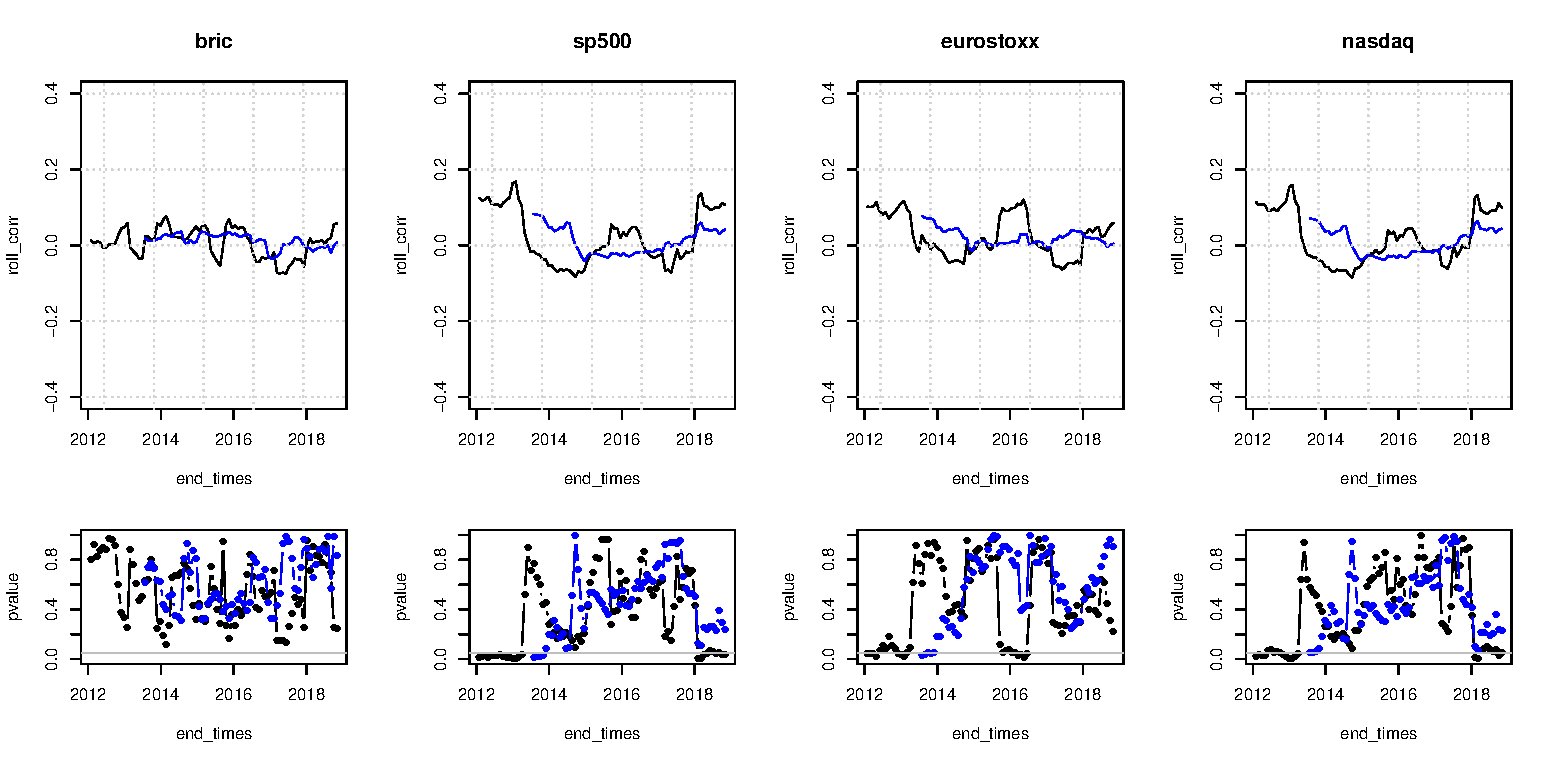
\includegraphics[width=14.5cm]{Images/images_samuele/rolling_stocks.pdf} %
		\bigskip
		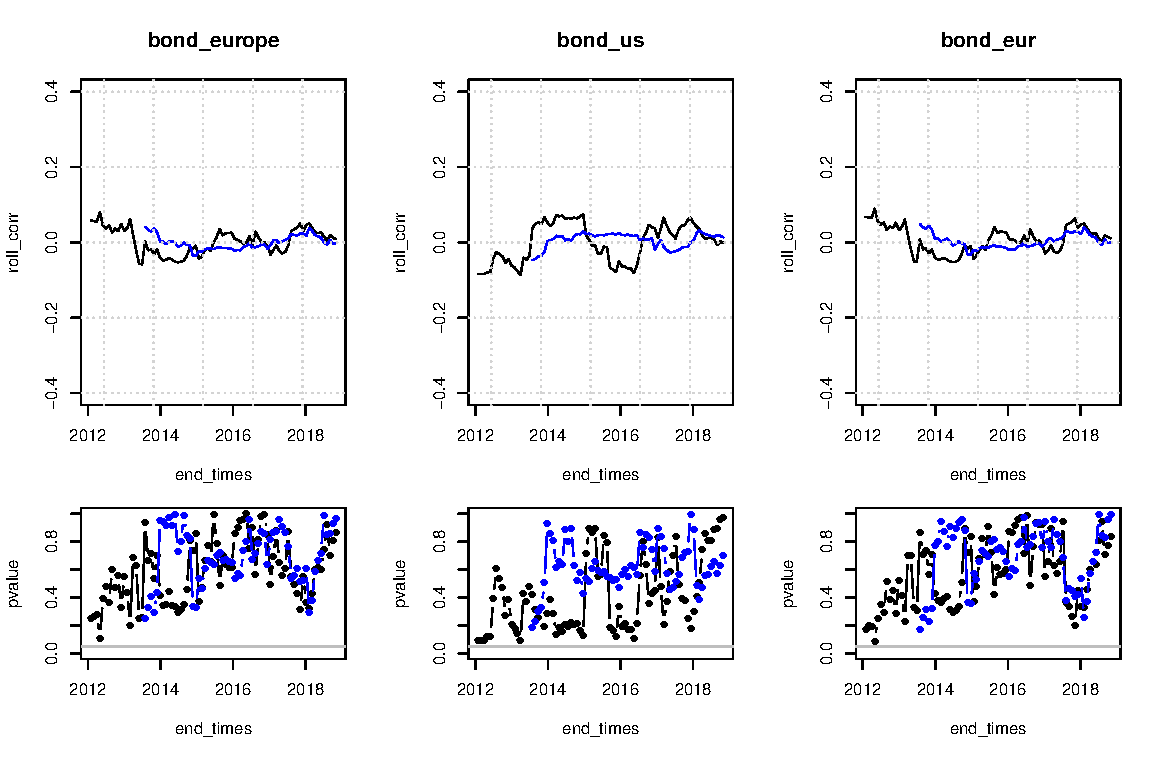
\includegraphics[width=14.5cm]{Images/images_samuele/rolling_bonds.pdf} %
\end{figure}
\begin{figure}[htpb]
		\centering
		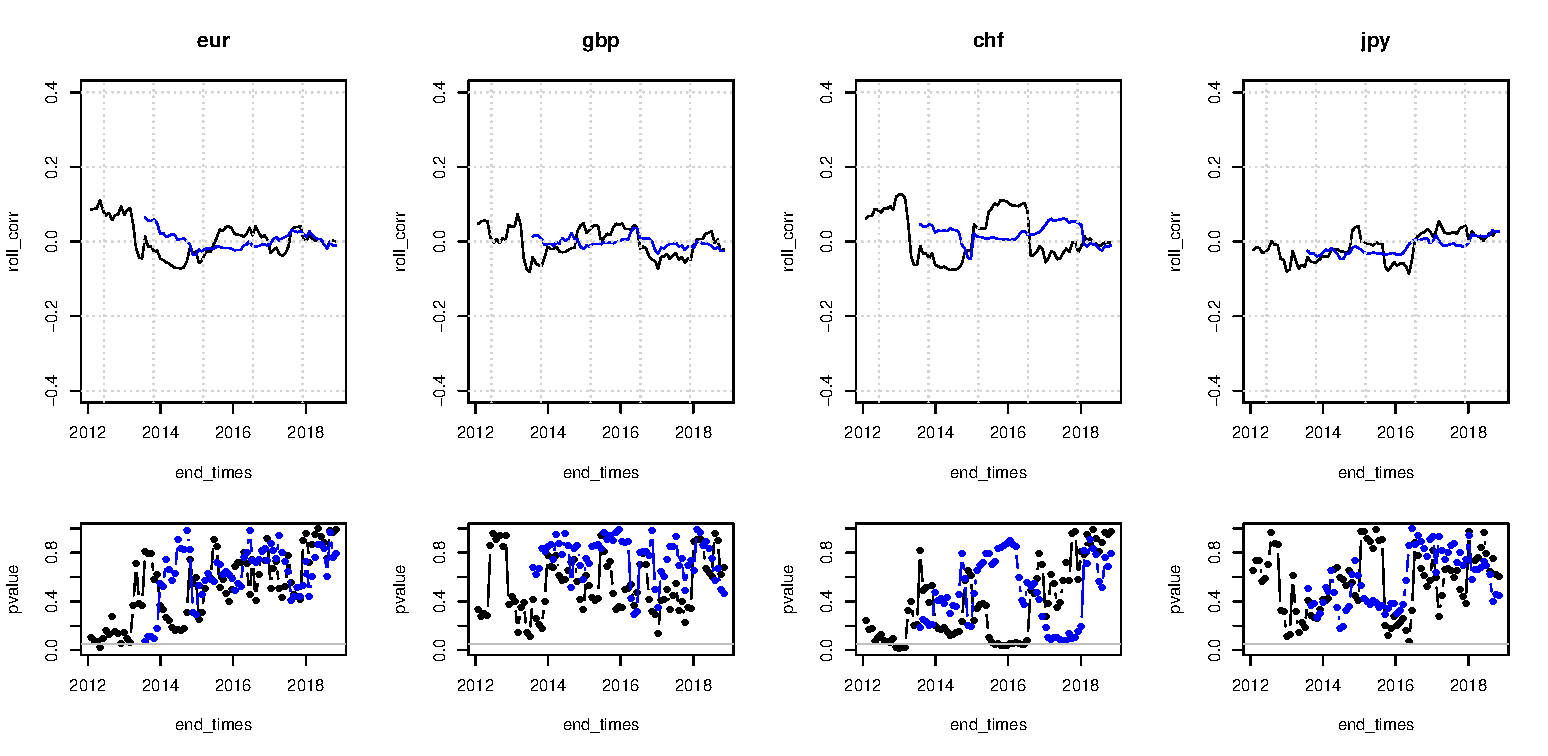
\includegraphics[width=14.5cm]{Images/images_samuele/rolling_fx.pdf} %
		\bigskip
		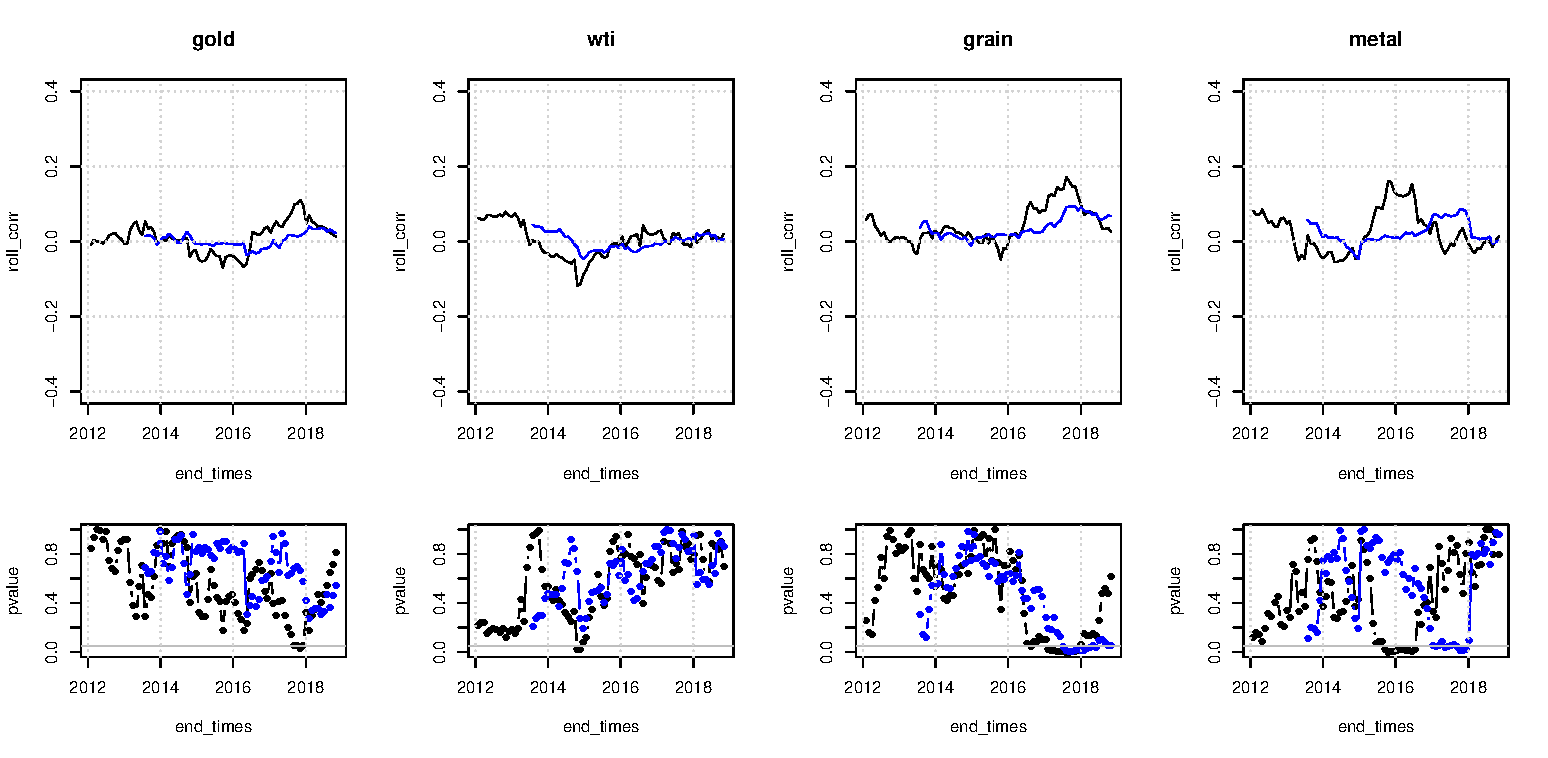
\includegraphics[width=14.5cm]{Images/images_samuele/rolling_commodities.pdf} %
		\caption{Rolling correlation between BTC and other instruments of the portfolio considered in \citep{samuele}}
		\label{samuele2}
\end{figure}

From these pictures one can immediately see that the correlation of any asset with Bitcoin is hardly ever significantly different from zero, and when it is, its absolute level is never greater than 15\% unless for a small period of time. Moreover, there is no line that is always above zero, nor below. This indicates that there is no underlying trend, whether positive or negative, and the correlation one might happen to find is only temporary.

Given these results the author try to understand the impact of including Bitcoin in an investment portfolio by drawing the efficient frontier using 2 different measures of risks: volatility and CVaR or expected shortfall.


\subsection{Mean-Variance method}


The first method used to draw the efficient frontier is the one introduced by Harry Markowitz in 1952.

It is the first mathematical framework which take into account the diversification principle in the field of asset allocation. Its key point is that an asset's return and risk should not be assessed by itself, but rather by how it affects the overall portfolio risk and return. To do so, the variance is used as a proxy for risk. Hence it is also called mean-variance analysis.

The main assumptions that are the building blocks of this theory are the following:
\begin{enumerate}
    \item investors are risk averse: they will always choose the less risky asset, when two assets offer the same return. At the same time, an investor wanting a higher return has to be willing to accept a higher risk. This equally holds for portfolios as a whole: given two portfolio with different risk profiles, he will choose the less risky in case of same return and the most remunerating in case of same risk;
    \item portfolio return is the weighted sum of the single assets' returns: in general, $E\left[ R_ptf\right] = \sum_{{i=1}}^{N} w_i E\left[ R_i\right]$;
    \item portfolio variance is a function of both the assets variances and their correlations: $V_ptf = \sum_{{i=1}}^{N}w_i \sigma_i^2 + \sum_{{i=1}}^{N} \sum_{{j \neq i, }{j = 1}}^{N} w_i w_j \rho_{i,j} \sigma_i \sigma_j $
\end{enumerate}
Now the optimization problem to be solved is:

\begin{equation*}
\begin{aligned}
& \underset{\text{w} \in R^N}{\text{minimize}}
& & & & \sigma_{ptf}^2\left(\text{w}\right) \\
& \text{subject to}
& & & & \text{e}^T \text{w} = 1 \text{,} \\
&&&&& \text{r}^T \text{w} = r_target \text{,} \\
&&&&& w_i \geq 0, for i = 1...N \text{.}
\end{aligned}
\end{equation*}

where e indicates a vector of ones and the first constraint makes sure that the sum of the weights always equals to one. This is to represent a portfolio in which all the money available is allocated in the assets we are taking into consideration. The second constraint ensures that the portfolio allocation $w$ produces the target expected return $r_target$. Finally, the last constraint is in fact optional and is only used to exclude the possibility to go short on any asset.

\begin{figure}[H]
		\centering
		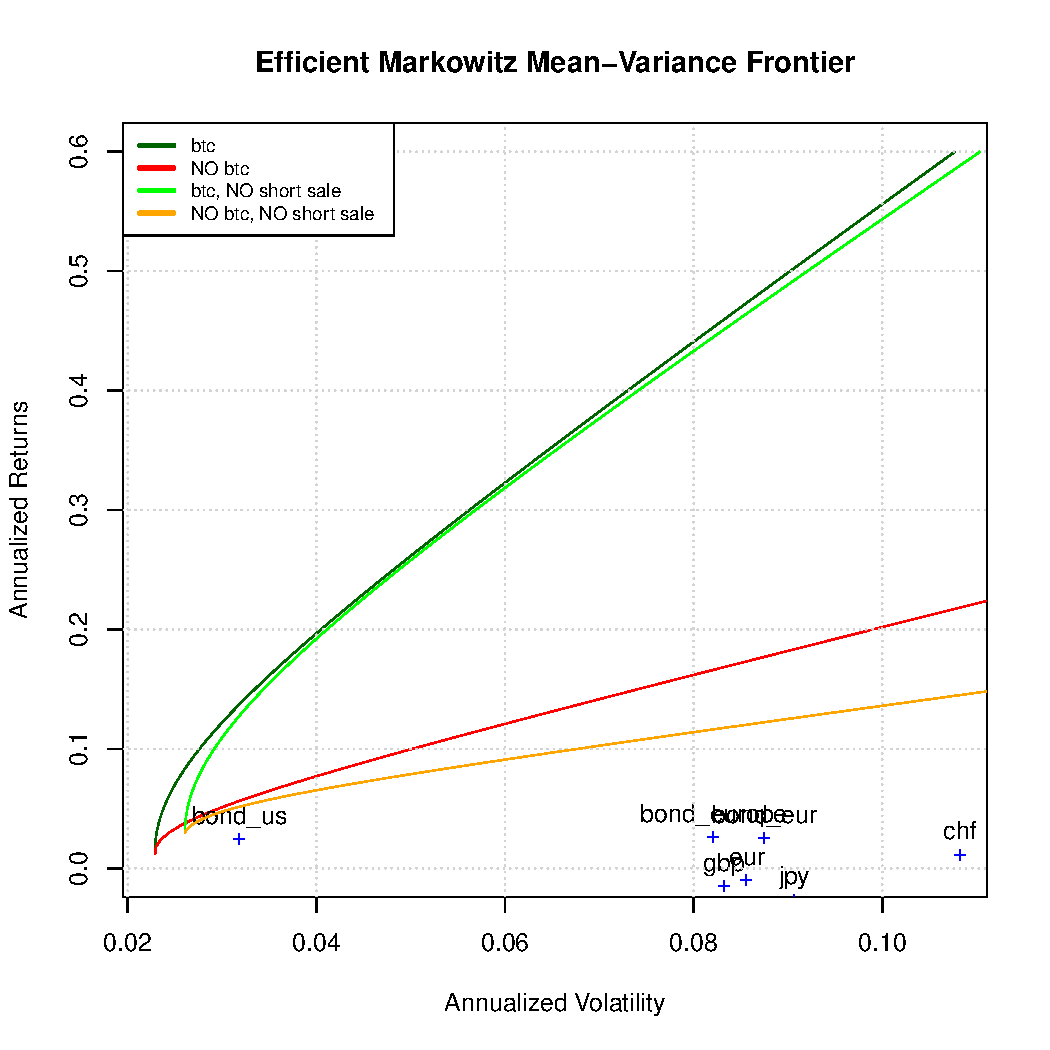
\includegraphics[width=13cm]{Images/images_samuele/efficient_frontier.pdf} %
        \caption{Efficient Frontier under Mean-Variance method, source: \citep{samuele}}
        \label{samuele3}
\end{figure}

In this framework, as shown n figure \ref{samuele3}, the efficient frontier with Bitcoin in the portfolio is much better than the one without Bitcoin, both in the case of no-short sale constraints and in the other case.
\newpage
In table \ref{tabsamuele1} the expected annualized returns of the portfolio reported from the author for different levels of volatility:

\begin{table}[H]
    \resizebox{\textwidth}{!}{\begin{tabular}{c c c}
        Volatility Level & Return without Bitcoin & Return including Bitcoin\\ \hline
        2.61\% & 3.00\% & 3.00\%\\
        2.75\% & 3.89\% & 7.70\%\\
        3.00\% & 4.59\% & 10.94\%\\
        3.25\% & 5.05\% & 13.37\%\\
        3.50\% & 5.43\% & 15.48\%\\
        3.75\% & 5.76\% & 17.41\%\\
        4.00\% & 6.06\% & 19.21\%\\
        4.25\% & 6.34\% & 20.94\%\\
        4.50\% & 6.61\% & 22.60\%\\
        4.75\% & 6.87\% & 24.21\%\\
        5.00\% & 7.12\% & 25.79\%\\
        5.25\% & 7.37\% & 27.34\%\\
        5.50\% & 7.61\% & 28.86\%\\
        5.75\% & 7.85\% & 30.37\%\\
        6.00\% & 8.08\% & 31.85\%\\
        \hline
    \end{tabular}}
    \caption{Results under Mean-Variance optimization, source: \citep{samuele}}
    \label{tabsamuele1}
\end{table}
\bigskip
\subsection{CVaR method}


Then the author studies the allocation in a slightly different framework: by using as risk measure of the portfolio the CVaR (conditional VaR).

To use this approach it is required only to change the objective function with no alterations on the constraints. The formulation of the problem become the following:

\begin{equation*}
\begin{aligned}
& \underset{\text{w} \in R^N}{\text{minimize}}
& & & & PtfRisk\left(\text{w}\right) \\
& \text{subject to}
& & & & \text{e}^T \text{w} = 1 \text{,} \\
&&&&& \text{r}^T \text{w} = r_target \text{,} \\
&&&&& w_i \geq 0, for i = 1...N \text{.}
\end{aligned}
\end{equation*}

where the $PtfRisk \left( \text{w} \right)$ is defined as:
\begin{equation}
    CVaR = \frac{1}{1-\alpha} \int_{\alpha}^1 VaR_\gamma d\gamma ,
\end{equation}


The introduction of this method is justified by the author by saying that the classic mean-variance framework, which consider the volatility as a proxy for the portfolio risk, does not distinguish between the volatility part caused by positive and negative returns. High returns yield higher volatility and so are penalized. The CVaR method solve this problem since it considers the loss distribution of the portfolio, and so just negative returns yield penalization to an asset.

The previous results are confirmed: the efficient frontier of the portfolio which includes Bitcoin is better than the one without Bitcoin also in this analytical framework.

\begin{figure}[H]
    \centering
    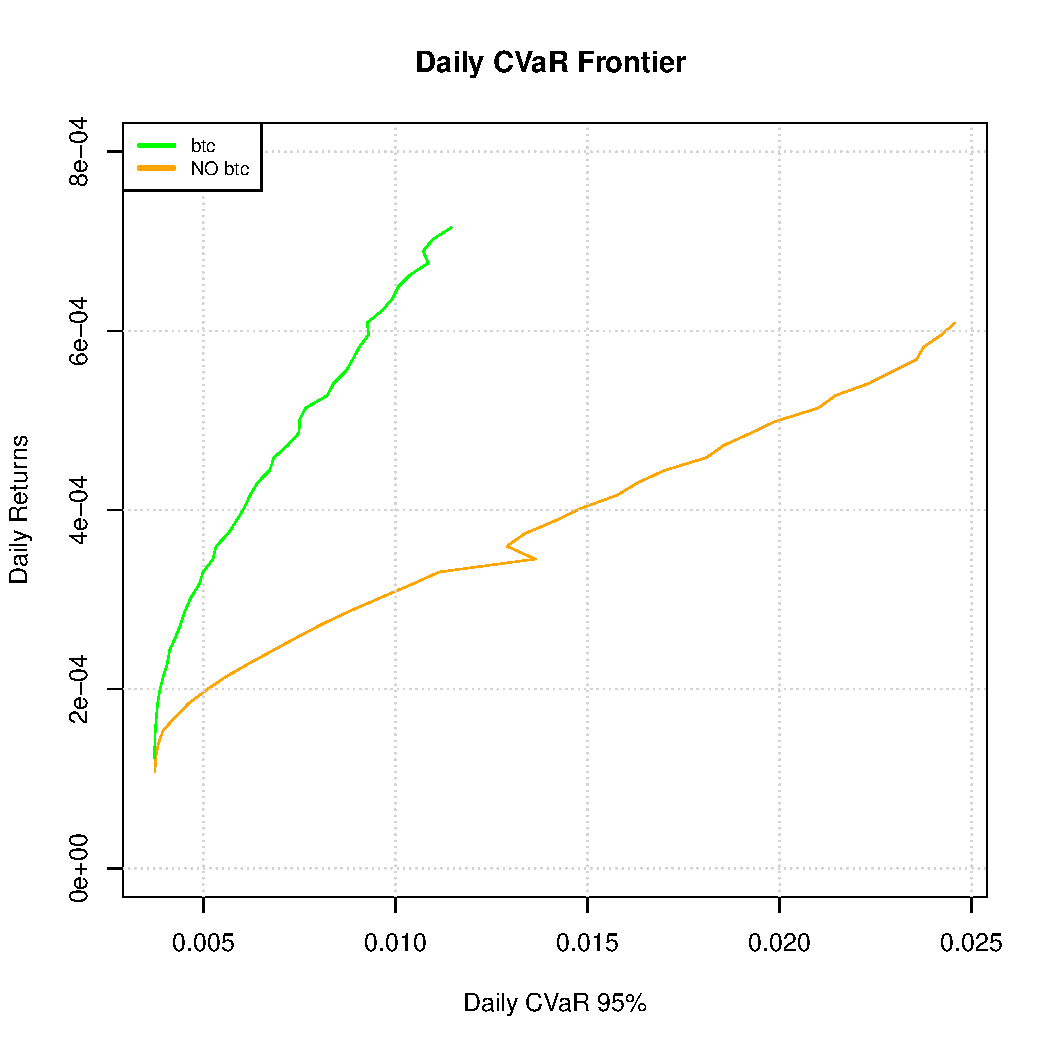
\includegraphics[width=13cm]{Images/images_samuele/efficient_frontier_CVaR.pdf}
    \caption{Efficient Frontier under CVaR method, source: \citep{samuele}}
\end{figure}

The results of this work lead to think of Bitcoin as a useful diversification instrument: it is uncorrelated to all the other instruments and it produces high returns.

